\section{RQ3: Physics-Informed Features}
\label{sec:rq3}

Nineteen candidates were computed from cycles $\le100$ and screened on the
41 training cells only:
\begin{itemize}
  \item \textbf{Mechanism signatures:} change of the main dQ/dV peak (height,
  voltage, area), charge recovered in the 2.0\,V hold, offset of $\dq$ at
  2\,V, coulombic-efficiency deficit, resistance growth and temperature rise.
  \item \textbf{Shape of the fade:} curvature of the capacity curve, exponent
  of the growth of $\Delta Q_{n-10}(V)$, and a $\dq$ variance averaged over
  several cycles.
  \item \textbf{Policy and procedure:} plating index of the policy,
  temperature at the start of the fast charge, cycle duration.
  \item \textbf{Early capacity rise (anode overhang):} rise before and after
  cycle 10, cycle of the peak, time to half rise.
  \item \textbf{Capacity budget:} \texttt{margin\_rate}, the capacity above
  end of life divided by the degradation rate.
\end{itemize}
A candidate had to add information within each training batch ($t$-statistic
of its coefficient in a linear fit with $\log_{10}\mathrm{Var}(\dq)$), keep
the same sign in b1 and b2, lower the cross-validated error, and still help
on top of a batch label.

\begin{table}[!htb]
\centering
\caption{Screening on the training cells (10 of 19 candidates). $\rho$:
Spearman correlation with $\log_{10}$ life; $t$: $t$-statistic of the
candidate in a linear fit with $\log_{10}\mathrm{Var}(\dq)$, within each batch
($|t|>2.1\approx p<0.05$); Gain: change in CV error when added (\%, positive
= better), alone and on top of a batch label. Bold: passed all criteria.}
\label{tab:screen}
\small
\setlength{\tabcolsep}{2.2pt}
\begin{tabular}{@{}lrrrrr@{}}
\toprule
Candidate & $\rho$ & $t$ b1 & $t$ b2 & Gain & +batch \\
\midrule
dQ/dV peak area change & $+0.77$ & $-1.6$ & $+2.0$ & $-3.6$ & $-2.6$ \\
CV-hold charge at 2.0\,V & $-0.72$ & $+1.9$ & $-2.6$ & $-4.1$ & $-4.7$ \\
Resistance slope vs.\ $\sqrt N$ & $+0.30$ & $+1.8$ & $-2.8$ & $-1.4$ & $+2.7$ \\
Curvature of fade & $+0.53$ & $+2.9$ & $+1.4$ & $-7.4$ & $-5.5$ \\
Exponent of $\Delta Q$ growth & $-0.39$ & $-1.4$ & $+0.6$ & $-0.7$ & $+1.9$ \\
Plating index of policy & $-0.62$ & $+0.8$ & $+2.7$ & $-2.7$ & $+7.6$ \\
Cycle duration & $-0.69$ & $+0.6$ & $-0.7$ & $+24.8$ & $+2.2$ \\
Capacity rise, cycles 2--10 & $+0.20$ & $-2.6$ & $-0.7$ & $+6.4$ & $+3.1$ \\
\textbf{Capacity rise after 10} & $-0.06$ & $-3.9$ & $-1.6$ & $+25.7$ & $+11.2$ \\
\textbf{Margin / rate} & $+0.83$ & $+5.3$ & $+0.1$ & $+9.6$ & $-0.3$ \\
\bottomrule
\end{tabular}
\end{table}

\subsection{Screening results}
\textbf{Mechanism features add nothing.} The dQ/dV, CV-hold, efficiency and
resistance features all increase the cross-validated error
(Table~\ref{tab:screen}). They are computed from the same curves, and $\dq$
already sums the effect of every mechanism.

\textbf{Several features only identify the batch.} Cycle duration lowers the
CV error by 25\,\% on its own but only 2\,\% once the batch is known. The
curvature of the fade correlates with life at $\rho=+0.53$ overall but
$-0.36$ in b1 and $+0.39$ in b2. The plating index of the policy
correlates at $\rho=-0.62$ overall but not within either batch (0.02,
0.03).

\textbf{The fade shows no early acceleration.} In most training cells the
amplitude of $\Delta Q_{n-10}(V)$ grows linearly with $n-10$ (median exponent
1.01, interquartile range 0.98--1.11; Fig.~\ref{fig:rq3}a). The knee cannot be seen in the first 100 cycles,
so curvature and acceleration features carry no extra signal.

\textbf{Two quantities passed the criteria, but neither adds a usable
signal.} (Two timing variants of the overhang rise, the peak and half-rise
cycles, also passed; they carry the same information as
\texttt{overhang\_after10}, $\rho=0.77$--0.89, and are weaker.)
\begin{itemize}
  \item \texttt{margin\_rate}, the capacity left before end of life over the
  degradation rate:
  \begin{align*}
  &\log_{10}\frac{Q_{d,2}-0.88\,\mathrm{Ah}}{\mathrm{sd}(\dq)}\\
  &\quad=\log_{10}(Q_{d,2}-0.88)-\tfrac12\log_{10}\mathrm{Var}(\dq),
  \end{align*}
  and it correlates with $\log_{10}\mathrm{Var}(\dq)$ at $r=-0.995$
  (Fig.~\ref{fig:rq3}b). Its only added information is the initial capacity
  $Q_{d,2}$, which F2 already contains: a free linear fit of
  $\log_{10}\mathrm{Var}(\dq)$ and $Q_{d,2}$ gives the same CV error (0.0635
  vs.\ 0.0649 in $\log_{10}$ life). It is therefore not used.
  \item \texttt{overhang\_after10}, the rise of the 9-cycle rolling median of
  capacity from cycle 10 to its maximum within cycles 2--100
  (Fig.~\ref{fig:rq3}c). Given $\dq$, cells with a
  larger late rise live somewhat shorter ($t=-3.9$ in b1, $-1.6$ in b2;
  Fig.~\ref{fig:rq3}d), consistent with lithium released inside the $\dq$
  window hiding some degradation.
\end{itemize}

\begin{figure}[!htb]
  \centering
  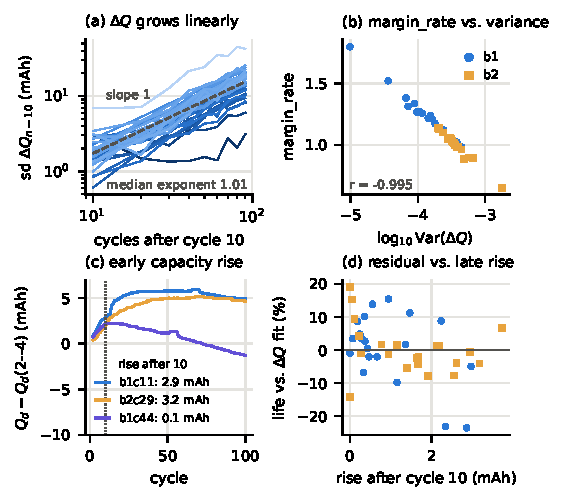
\includegraphics[width=\columnwidth]{fig_rq3_physics}
  \caption{Training cells. (a) Amplitude of $\Delta Q_{n-10}(V)$ (log axes,
  darker = longer life). (b) \texttt{margin\_rate} against
  $\log_{10}\mathrm{Var}(\dq)$. (c) Early capacity of three cells (9-cycle
  rolling median); dotted: cycle 10. (d) Life relative to a $\dq$-only fit
  within each batch, against the rise after cycle 10.}
  \label{fig:rq3}
\end{figure}

\subsection{Does the overhang rise help?}
\texttt{overhang\_after10} was added to F1 and F2 and the elastic net was
evaluated once on all test sets (Table~\ref{tab:overhang}).

\begin{table}[!htb]
\centering
\caption{Elastic net with and without \texttt{overhang\_after10} (OH): CV
error ($\log_{10}$ life, training cells) and test RMSE (cycles). In range:
primary cells inside the training life range.}
\label{tab:overhang}
\small
\setlength{\tabcolsep}{3.5pt}
\begin{tabular}{@{}lccccc@{}}
\toprule
Set & CV & Primary & In range & Secondary & u1 \\
\midrule
F1 & .0717 & 138 & 108 & 196 & 119 \\
F1 + OH & .0536 & 126 & 89 & 205 & 179 \\
\midrule
F2 & .0578 & 90 & 86 & 167 & 260 \\
F2 + OH & .0530 & 113 & 79 & 174 & 189 \\
\bottomrule
\end{tabular}
\end{table}

Within the training batches the rise helps: it lowers the CV error by 25\,\%
on top of F1 and 8\,\% on top of F2, and improves the in-range primary error
(F1: $-19$ cycles, bootstrap interval $-32$ to $-7$; F2: $-7$, $-14$ to $+2$).
On a new batch it does not: on the secondary set both versions are slightly
worse ($+12$ and $+6$, intervals include zero), and on u1 it makes F1
significantly worse ($+60$, $+26$ to $+89$) but F2 better ($-70$, $-93$ to
$-44$). The u1 standard cells have rises of up to 10.8\,mAh against at most
3.7\,mAh in training, so the linear term extrapolates far; with F2 it probably
offsets an over-prediction caused by the capacity features
(Section~\ref{sec:rq5}). An effect that changes sign with the feature set is
not a reliable signal, so the overhang rise is not used either.

\textbf{Answer to RQ3.} No. Mechanism features are redundant with $\dq$,
several candidates only identify the batch, \texttt{margin\_rate} recombines
$\dq$ and $Q_{d,2}$, and the overhang rise helps only within the training
batches. All later sections use F1--F3.
